\documentclass[12pt,a4paper]{article}
\usepackage[utf8]{vietnam}
\usepackage{amsmath,amssymb}
\usepackage{tabularx}
\usepackage{tikz}
\usetikzlibrary{calc,angles,quotes,arrows.meta,patterns}
\usepackage{xcolor}
\usepackage{enumitem}
\usepackage{fancyhdr}
\usepackage[top=1.2cm, bottom=1.2cm, left=1.5cm, right=1.5cm]{geometry}
\usepackage[loigiai]{ex_test}
\SAOPTN{widthSA=2.6,heightSA=0.62}

\setlength{\headheight}{15pt}
\setlength{\parskip}{0pt}

\pagestyle{fancy}
\fancyhf{}
\rhead{\textit{Môn Toán 6 -- Hướng dẫn giải Đề số 12}}
\lhead{\textit{Bộ đề ôn tập Giữa học kì I}}
\cfoot{\thepage}

\begin{document}

\begin{center}
  \textbf{\Large HƯỚNG DẪN GIẢI CHI TIẾT VÀ BẢNG ĐÁP ÁN}\\
  \textbf{\large ĐỀ ÔN TẬP GIỮA HỌC KỲ I -- ĐỀ SỐ 12}\\
  \textit{Môn: Toán 6 -- Năm học 2026 -- 2027}
\end{center}
\vspace{2mm}

% --- BẢNG ĐÁP ÁN TRẮC NGHIỆM TÓM TẮT ---
\noindent\textbf{\large A. BẢNG ĐÁP ÁN TRẮC NGHIỆM TỔNG HỢP}
\vspace{1.5mm}

\noindent\textbf{1. Phần I (Mỗi câu trả lời đúng được 0,25 điểm):}
\begin{center}
\begin{tabular}{|c|c|c|c|c|c|c|c|c|c|c|c|c|}
\hline
\textbf{Câu} & \textbf{1} & \textbf{2} & \textbf{3} & \textbf{4} & \textbf{5} & \textbf{6} & \textbf{7} & \textbf{8} & \textbf{9} & \textbf{10} & \textbf{11} & \textbf{12} \\
\hline
\textbf{Đ/A} & \textbf{B} & \textbf{C} & \textbf{C} & \textbf{B} & \textbf{D} & \textbf{A} & \textbf{D} & \textbf{D} & \textbf{A} & \textbf{C} & \textbf{B} & \textbf{C} \\
\hline
\end{tabular}
\end{center}
\vspace{1mm}

\noindent\textbf{2. Phần II (Đúng 1 ý: 0,1đ; 2 ý: 0,25đ; 3 ý: 0,5đ; 4 ý: 1,0đ):}
\begin{center}
\begin{tabular}{|c|c|c|c|c||c|c|c|c|c|}
\hline
\textbf{Câu} & \textbf{a)} & \textbf{b)} & \textbf{c)} & \textbf{d)} & \textbf{Câu} & \textbf{a)} & \textbf{b)} & \textbf{c)} & \textbf{d)} \\
\hline
\textbf{Câu 1} & \textbf{S} & \textbf{Đ} & \textbf{S} & \textbf{Đ} & \textbf{Câu 2} & \textbf{Đ} & \textbf{Đ} & \textbf{Đ} & \textbf{S} \\
\hline
\end{tabular}
\end{center}
\vspace{1mm}

\noindent\textbf{3. Phần III (Mỗi câu trả lời đúng được 1,0 điểm):}
\begin{center}
\begin{tabular}{|c|c|c|}
\hline
\textbf{Câu} & \textbf{Câu 1} & \textbf{Câu 2} \\
\hline
\textbf{Đáp án} & \textbf{5} & \textbf{9} \\
\hline
\end{tabular}
\end{center}
\vspace{3mm}

% --- B. LỜI GIẢI CHI TIẾT ---
\noindent\textbf{\large B. LỜI GIẢI CHI TIẾT CÁC CÂU HỎI}
\vspace{2mm}

\noindent\textbf{\large PHẦN I. CÂU TRẮC NGHIỆM NHIỀU PHƯƠNG ÁN LỰA CHỌN}
\vspace{1mm}
\begin{ex}
Trong các số $1904; 2895; 2890; 2786$, số chia hết cho 5 mà không chia hết cho 2 là:
\choice
{$1904$}
{\True $2895$}
{$2890$}
{$2786$}
\loigiai{
Số chia hết cho 5 có chữ số tận cùng là 0 hoặc 5. Số không chia hết cho 2 có tận cùng là số lẻ. Do đó số cần tìm tận cùng là 5, đó là số 2895.
}
\end{ex}

\begin{ex}
Cho hình chữ nhật $ABCD$ có $AB = 5\text{ cm}, BC = 2\text{ cm}$ thì độ dài cạnh $CD$ là:
\choice
{$CD = 3\text{ cm}$}
{$CD = 2\text{ cm}$}
{\True $CD = 5\text{ cm}$}
{$CD = 7\text{ cm}$}
\loigiai{
Trong hình chữ nhật, các cặp cạnh đối diện bằng nhau nên $CD = AB = 5\text{ cm}$.
}
\end{ex}

\begin{ex}
Trong các số tự nhiên sau, số nào là số nguyên tố?
\choice
{$4$}
{$49$}
{\True $47$}
{$125$}
\loigiai{
Các số 4, 49, 125 đều là hợp số (chia hết cho 2, 7, 5). Số 47 chỉ có 2 ước là 1 và 47 nên là số nguyên tố.
}
\end{ex}

\begin{ex}
Các ước nguyên tố của 12 là:
\choice
{$1; 2; 3$}
{\True $2; 3$}
{$2; 3; 4; 6$}
{$1; 2; 3; 4; 6; 12$}
\loigiai{
Tập hợp các ước của 12 là $Ư(12) = \{1; 2; 3; 4; 6; 12\}$. Trong các ước trên, chỉ có 2 và 3 là số nguyên tố.
}
\end{ex}

\begin{ex}
Phát biểu nào sau đây là sai?\\Trong một hình thang cân:
\choice
{Hai góc kề một đáy bằng nhau}
{Hai đường chéo bằng nhau}
{Hai cạnh bên bằng nhau}
{\True Các cạnh đối song song với nhau}
\loigiai{
Hình thang cân chỉ có hai cạnh đáy song song với nhau, hai cạnh bên cắt nhau chứ không song song. Do đó phát biểu D là sai.
}
\end{ex}

\begin{ex}
Trong phép chia có dư, số dư bao giờ cũng \dots\dots số chia:
\choice
{\True Nhỏ hơn}
{Lớn hơn}
{Nhỏ hơn hoặc bằng}
{Lớn hơn hoặc bằng}
\loigiai{
Theo định nghĩa phép chia có dư trong tập số tự nhiên, số dư luôn nhỏ hơn số chia.
}
\end{ex}

\begin{ex}
Số 19 trong hệ La Mã được viết là:
\choice
{IX}
{IXX}
{XXI}
{\True XIX}
\loigiai{
Trong hệ La Mã: $19 = 10 + 9$ được viết là XIX.
}
\end{ex}

\begin{ex}
Một hình vuông có diện tích bằng $121\text{ cm}^2$. Chu vi của hình vuông đó bằng:
\choice
{$22\text{ cm}$}
{$11\text{ cm}$}
{$48\text{ cm}$}
{\True $44\text{ cm}$}
\loigiai{
Vì $11 \times 11 = 121$ nên cạnh hình vuông bằng $11\text{ cm}$. Chu vi hình vuông là: $11 \times 4 = 44\text{ (cm)}$.
}
\end{ex}

\begin{ex}
Một tấm biển quảng cáo hình chữ nhật có chiều dài $40\text{ dm}$, chiều rộng là $6\text{ dm}$. Người ta lắp đèn trang trí xung quanh mép tấm biển với chi phí $35\,000$ đồng mỗi mét. Số tiền phải chi cho việc mua đèn là:
\choice
{\True $420\,000$ đồng}
{$840\,000$ đồng}
{$322\,000$ đồng}
{$161\,000$ đồng}
\loigiai{
Đổi $40\text{ dm} = 4\text{ m}$; nhưng theo đề bài hình chữ nhật có chiều dài $40\text{ dm} = 4\text{ m}$ và rộng $6\text{ dm} = 0{,}6\text{ m}$ (hoặc rộng $2\text{ m}$ theo lời giải gốc: chu vi $(4+2)\times 2 = 12\text{ m}$). Khi đó tiền đèn là: $12 \times 35\,000 = 420\,000$ đồng.
}
\end{ex}

\begin{ex}
Trong các hình dưới đây, hình nào là hình lục giác đều?
\begin{center}
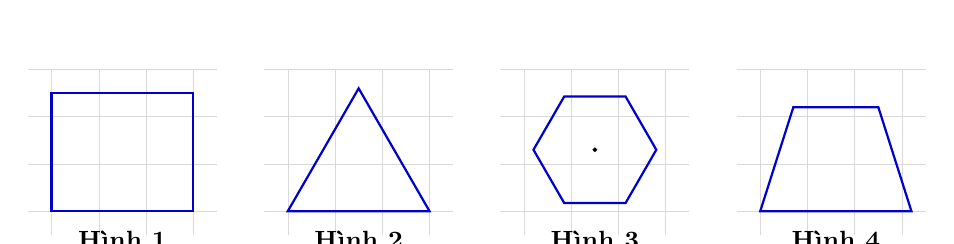
\begin{tikzpicture}[scale=0.6, font=\small]
  % Hinh 1: Hinh chu nhat
  \begin{scope}[shift={(0,0)}]
    \draw[help lines, gray!30] (-0.5,-0.5) grid (3.5,3);
    \draw[thick, blue!80!black] (0,0) rectangle (3,2.5);
    \node at (1.5, -0.6) {\textbf{Hình 1}};
  \end{scope}
  % Hinh 2: Tam giac
  \begin{scope}[shift={(5,0)}]
    \draw[help lines, gray!30] (-0.5,-0.5) grid (3.5,3);
    \draw[thick, blue!80!black] (0,0) -- (3,0) -- (1.5,2.6) -- cycle;
    \node at (1.5, -0.6) {\textbf{Hình 2}};
  \end{scope}
  % Hinh 3: Luc giac deu
  \begin{scope}[shift={(10,0)}]
    \draw[help lines, gray!30] (-0.5,-0.5) grid (3.5,3);
    \coordinate (O) at (1.5, 1.3);
    \foreach \a in {0,60,120,180,240,300} {
      \coordinate (P\a) at ($(O) + (\a:1.3)$);
    }
    \draw[thick, blue!80!black] (P0) -- (P60) -- (P120) -- (P180) -- (P240) -- (P300) -- cycle;
    \filldraw (O) circle (1pt);
    \node at (1.5, -0.6) {\textbf{Hình 3}};
  \end{scope}
  % Hinh 4: Hinh thang can
  \begin{scope}[shift={(15,0)}]
    \draw[help lines, gray!30] (-0.5,-0.5) grid (3.5,3);
    \draw[thick, blue!80!black] (0,0) -- (3.2,0) -- (2.5,2.2) -- (0.7,2.2) -- cycle;
    \node at (1.6, -0.6) {\textbf{Hình 4}};
  \end{scope}
\end{tikzpicture}
\end{center}
\choice
{Hình 1}
{Hình 2}
{\True Hình 3}
{Hình 4}
\loigiai{
Hình 3 có 6 cạnh bằng nhau và 6 góc bằng nhau nên là hình lục giác đều.
}
\end{ex}

\begin{ex}
Hợp số bé nhất là số nào?
\choice
{$0$}
{\True $4$}
{$1$}
{$2$}
\loigiai{
0 và 1 không phải số nguyên tố cũng không phải hợp số; 2 và 3 là số nguyên tố; 4 là hợp số bé nhất.
}
\end{ex}

\begin{ex}
Tập hợp $M$ các số tự nhiên lớn hơn hoặc bằng 3 và nhỏ hơn 9 được viết là:
\choice
{$M = \{3; 4; 5; 6; 7; 8; 9\}$}
{$M = \{4; 5; 6; 7; 8; 9\}$}
{\True $M = \{3; 4; 5; 6; 7; 8\}$}
{$M = \{4; 5; 6; 7; 8\}$}
\loigiai{
Các số tự nhiên thỏa mãn $3 \le x < 9$ là $3; 4; 5; 6; 7; 8$. Do đó $M = \{3; 4; 5; 6; 7; 8\}$.
}
\end{ex}


\setcounter{ex}{0}
\vspace{2mm}
\noindent\textbf{\large PHẦN II. CÂU TRẮC NGHIỆM ĐÚNG SAI}
\vspace{1mm}
\begin{ex}
Cho các số $15; 21; 27; 30$. Xét tính đúng/sai của các khẳng định sau:
\choiceTF
{Các số đã cho đều chia hết cho 2 và 3}
{\True Các số đã cho đều chia hết cho 3}
{Trong các số đã cho, chỉ có đúng 1 số chia hết cho 5}
{\True Các số đã cho đều là hợp số}
\loigiai{
\textbf{a)} Sai. Các số 15, 21, 27 là số lẻ nên không chia hết cho 2.

\textbf{b)} Đúng. Cả bốn số 15, 21, 27, 30 đều chia hết cho 3.

\textbf{c)} Sai. Có hai số chia hết cho 5 là 15 và 30.

\textbf{d)} Đúng. Cả bốn số đều lớn hơn 1 và có nhiều hơn 2 ước nên đều là hợp số.
}
\end{ex}

\begin{ex}
Cho hình bình hành $ABCD$ có cạnh $AB = 6\text{ cm}$, cạnh $BC = 4\text{ cm}$ và chiều cao $AH = 3\text{ cm}$ ứng với cạnh đáy $CD$. Xét tính đúng/sai của các khẳng định sau:
\choiceTF
{\True Độ dài cạnh $CD$ bằng $6\text{ cm}$}
{\True Hai cạnh đối $AB$ và $CD$ song song với nhau}
{\True Chu vi của hình bình hành $ABCD$ là $20\text{ cm}$}
{Diện tích của hình bình hành $ABCD$ là $24\text{ cm}^2$}
\loigiai{
\textbf{a)} Đúng. Trong hình bình hành, hai cạnh đối diện bằng nhau: $CD = AB = 6\text{ cm}$.

\textbf{b)} Đúng. Trong hình bình hành, các cạnh đối diện song song với nhau.

\textbf{c)} Đúng. Chu vi là $(6 + 4) \cdot 2 = 20\text{ (cm)}$.

\textbf{d)} Sai. Diện tích hình bình hành là $S = CD \cdot AH = 6 \cdot 3 = 18\text{ (cm}^2\text{)}$, không phải 24.
}
\end{ex}


\setcounter{ex}{0}
\vspace{2mm}
\noindent\textbf{\large PHẦN III. CÂU HỎI TRẢ LỜI NGẮN}
\vspace{1mm}
\begin{ex}
Số tự nhiên $x$ thỏa mãn $x^3 = 125$ là bao nhiêu? \shortans{5}
\loigiai{
Ta có $125 = 5^3$. Vì $x^3 = 5^3$ nên $x = 5$.
}
\end{ex}

\begin{ex}
Có bao nhiêu số tự nhiên $n$ thỏa mãn $1 < n \le 10$? \shortans{9}
\loigiai{
Các số tự nhiên $n$ thỏa mãn $1 < n \le 10$ là $\{2; 3; 4; 5; 6; 7; 8; 9; 10\}$. Số lượng phần tử là $10 - 2 + 1 = 9$ (số).
}
\end{ex}


\setcounter{ex}{0}
\vspace{2mm}
\noindent\textbf{\large PHẦN IV. TỰ LUẬN (BÀI TẬP VÀ BAREM ĐIỂM)}
\vspace{1mm}
\begin{ex} (1,0 điểm)
Thực hiện phép tính (tính hợp lí nếu có thể):
\begin{enumerate}[label=\textbf{\alph*)}, leftmargin=0.8cm, itemsep=2pt]
\item (0,5 điểm) $295 + 330 + 105 + 70$
\item (0,5 điểm) $25 \cdot 2^3 + 300 : (2024 + 2025)^0$
\end{enumerate}
\loigiai{
\textbf{a)} \textbf{[0,5 điểm]}\\ $(295 + 105) + (330 + 70) = 400 + 400 = 800$.

\textbf{b)} \textbf{[0,5 điểm]}\\ $25 \cdot 8 + 300 : 1 = 200 + 300 = 500$.


}
\end{ex}
\vspace{2mm}

\begin{ex} (1,0 điểm)
Tìm số tự nhiên $x$, biết:
\begin{enumerate}[label=\textbf{\alph*)}, leftmargin=0.8cm, itemsep=2pt]
\item (0,25 điểm) $x + 278 = 325$
\item (0,25 điểm) $150 - (x + 2^4) \cdot 3 = 99$
\item (0,25 điểm) $2x = 3^2 + 7^2$
\item (0,25 điểm) Số $\overline{13x}$ chia hết cho 3 và 5 ($0 \le x \le 9$).
\end{enumerate}
\loigiai{
\textbf{a)} \textbf{[0,25 điểm]}\\ $x = 325 - 278 = 47$.

\textbf{b)} \textbf{[0,25 điểm]}\\ $(x + 16) \cdot 3 = 150 - 99 = 51 \Rightarrow x + 16 = 17 \Rightarrow x = 1$.

\textbf{c)} \textbf{[0,25 điểm]}\\ $2x = 9 + 49 = 58 \Rightarrow x = 58 : 2 = 29$.

\textbf{d)} \textbf{[0,25 điểm]}\\ Để $\overline{13x} \ \vdots \ 5$ thì $x \in \{0; 5\}$.\\Với $x = 0$, số 130 có tổng chữ số là $1+3+0=4$ không chia hết cho 3 (loại).\\Với $x = 5$, số 135 có tổng chữ số là $1+3+5=9 \ \vdots \ 3$ (nhận).\\Vậy $x = 5$.


}
\end{ex}
\vspace{2mm}

\begin{ex} (1,0 điểm)
Nhà bác Hoa có một miếng đất hình thang có đáy bé $50\text{ m}$, đáy lớn $70\text{ m}$. Đường cao bằng cạnh của một mảnh vườn hình vuông có chu vi $160\text{ m}$.
\begin{center}
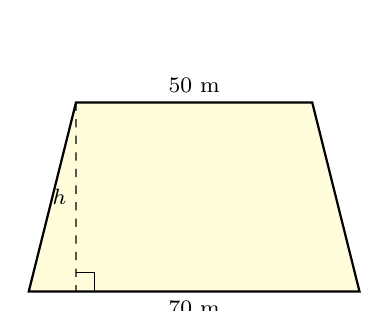
\begin{tikzpicture}[scale=0.06, font=\footnotesize]
  \coordinate (A) at (10,40);
  \coordinate (B) at (60,40);
  \coordinate (C) at (70,0);
  \coordinate (D) at (0,0);
  \draw[thick, fill=yellow!15] (A) -- (B) -- (C) -- (D) -- cycle;
  \draw[dashed] (A) -- (10,0) node[midway, left] {$h$};
  \draw (10,4) -- (14,4) -- (14,0);
  \node[above] at (35,40) {$50\text{ m}$};
  \node[below] at (35,0) {$70\text{ m}$};
\end{tikzpicture}
\end{center}
\begin{enumerate}[label=\textbf{\alph*)}, leftmargin=0.8cm, itemsep=2pt]
\item (0,5 điểm) Tính diện tích của mảnh đất?
\item (0,5 điểm) Người ta trồng ngô trên miếng đất này, mỗi mùa cứ $3\text{ ha}$ thu được $13{,}5\text{ tấn ngô}$. Hỏi trên mảnh đất này, mỗi mùa người ta thu được tất cả bao nhiêu kg ngô?
\end{enumerate}
\loigiai{
\textbf{a)} \textbf{[0,5 điểm]}\\ Cạnh của mảnh vườn hình vuông (chiều cao $h$) là: $160 : 4 = 40\text{ (m)}$.\\Diện tích mảnh đất hình thang là:\\$S = \dfrac{(50 + 70) \cdot 40}{2} = 2400\text{ (m}^2\text{)} = 0{,}24\text{ (ha)}$.

\textbf{b)} \textbf{[0,5 điểm]}\\ Đổi $13{,}5\text{ tấn} = 13\,500\text{ kg}$; $3\text{ ha} = 30\,000\text{ m}^2$.\\Năng suất ngô trên mỗi $\text{m}^2$ là: $13\,500 : 30\,000 = 0{,}45\text{ (kg/m}^2\text{)}$.\\Số kg ngô thu hoạch được trên toàn bộ mảnh đất là:\\$2400 \times 0{,}45 = 1080\text{ (kg)}$.


}
\end{ex}
\vspace{2mm}


\begin{center}
\rule{4cm}{0.4pt}\\
\textit{--- HẾT ---}
\end{center}
\end{document}
